\chapter{Flux de C\`{a}rregues}
\index{flux de c\`{a}rregues}\label{chap:flux_carregues}

Es tracta en aquest cap\'{\i}tol el m\`{e}tode de resoluci\'{o} del problema del flux de c\`{a}rregues en
sistemes el\`{e}ctrics de pot\`{e}ncia.

\section{Introducci\'{o}}

Quan les dades que es coneixen de les c\`{a}rregues d'una xarxa no s\'{o}n
les seves imped\`{a}ncies o admit\`{a}ncies, sin\'{o} les pot\`{e}ncies que
absorbeixen, no podem emprar el m\`{e}tode dels nusos, descrit en el
Cap\'{\i}tol \ref{chap:nusos}, per tal de resoldre la xarxa.

En aquest cas, el m\`{e}tode de resoluci\'{o} es basa en escriure per a cada
nus les equacions pertinents del balan\c{c} de pot\`{e}ncia activa i
reactiva, i resoldre-les. La soluci\'{o} del sistema d'equacions
resultant, ens proporcionar\`{a} les tensions de tots els nusos de la
xarxa, i el flux de pot\`{e}ncia activa i reactiva entre els seus nusos.

El sistema d'equacions que cal resoldre \'{e}s no lineal, i per tant,
cal emprar algun m\`{e}tode num\`{e}ric per a la seva resoluci\'{o}, com ara el
de Newton-Raphson;\index{Newton-Raphson} aqu\'{\i}, no obstant, no
s'explicar\`{a} cap m\`{e}tode num\`{e}ric de resoluci\'{o} de sistemes d'equacions
no lineals, ja que aix\`{o} cau fora de l'abast d'aquest llibre. Aix\`{o}
per\`{o}, no hauria de suposar cap problema, ja que avui dia aquests
sistemes d'equacions es poden resoldre f\`{a}cilment amb programes
d'ordinador de c\`{a}lcul matem\`{a}tic, com ara els programes
\textit{Mathematica}${}^\circledR$ o \textit{MATLAB}${}^\circledR$,
\index{Mathematica@\textit{Mathematica}${}^\circledR$}
\index{MATLAB@\textit{MATLAB}${}^\circledR$} o amb calculadores
cient\'{\i}fiques, com ara la calculadora \textsf{HP-49G}.

\section{Models matem\`{a}tics} \index{flux de c\`{a}rregues!models matem\`{a}tics}

En els estudis de flux de c\`{a}rregues, els elements que es consideren s\'{o}n:
\begin{dinglist}{'167}
   \item C\`{a}rregues
   \item L\'{\i}nies el\`{e}ctriques
   \item Transformadors amb regulaci\'{o} variable (amb decalatge o sense)
\end{dinglist}

\subsection{C\`{a}rregues}

Les c\`{a}rregues v\'{e}nen sempre definides per la pot\`{e}ncia que absorbeixen, \'{e}s a dir, es consideren fonts de pot\`{e}ncia constant.

\subsection{L\'{\i}nies el\`{e}ctriques} \index{linies@l\'{\i}nies el\`{e}ctriques}

Les l\'{\i}nies el\`{e}ctriques es modelen mitjan\c{c}ant un circuit equivalent
per fase en {"<}$\piup${">}, format per una imped\`{a}ncia longitudinal i dues
admit\`{a}ncies transversals, tal com es pot veure en la Figura
\vref{pic:equiv_linia}. En aquesta figura s'ha suposat que la l\'{\i}nia
est\`{a} connectada entre els nusos 1 i 2; les admit\`{a}ncies transversals,
tenen sempre un extrem connectat a terra (nus 0 de refer\`{e}ncia).
\index{linies@l\'{\i}nies el\`{e}ctriques!circuit equivalent en
\guillemotleft$\piup$\guillemotright}

\begin{figure}[htb]
\centering
    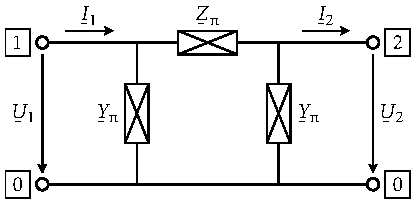
\includegraphics{Imatges/Cap-FluxCarregues-Linia.pdf}
\caption{Circuit equivalent d'una l\'{\i}nia el\`{e}ctrica}
\label{pic:equiv_linia}
\end{figure}

A partir dels par\`{a}metres propis d'una l\'{\i}nia: la seva imped\`{a}ncia
longitudinal  total per fase $\cmplx{Z}\ped{t}$ i la seva admit\`{a}ncia
transversal total per fase $\cmplx{Y}\ped{t}$, definim la imped\`{a}ncia
caracter\'{\i}stica $\cmplx{Z}\ped{c}$ i l'angle caracter\'{\i}stic
$\cmplx{\theta}\ped{c}$ de la l\'{\i}nia: \index{linies@l\'{\i}nies
el\`{e}ctriques!imped\`{a}ncia caracter\'{\i}stica} \index{linies@l\'{\i}nies
el\`{e}ctriques!angle caracter\'{\i}stic} \index{Zc@$\cmplx{Z}\ped{c}$}
\index{$\cmplx{\theta}\ped{c}$}
\begin{equation}
   \cmplx{Z}\ped{c} = \sqrt{\frac{\cmplx{Z}\ped{t}}{\cmplx{Y}\ped{t}}} \qquad \qquad
   \cmplx{\theta}\ped{c} = \sqrt{\cmplx{Z}\ped{t} \,\cmplx{Y}\ped{t} }
\end{equation}

Amb aquest dos par\`{a}metres, les equacions hiperb\`{o}liques de
transmissi\'{o} d'una l\'{\i}nia s\'{o}n: \index{linies@l\'{\i}nies
el\`{e}ctriques!equacions hiperb\`{o}liques de transmissi\'{o}}
\begin{equation}\label{eq:linia_eq_trans}
   \cmplx{U}_1 = \cmplx{U}_2 \cosh \cmplx{\theta}\ped{c}  + \cmplx{I}_2 \,\cmplx{Z}\ped{c} \sinh \cmplx{\theta}\ped{c}   \qquad \qquad
   \cmplx{I}_1 = \cmplx{U}_2 \, \frac{\sinh \cmplx{\theta}\ped{c}}{\cmplx{Z}\ped{c}}  +   \cmplx{I}_2 \cosh \cmplx{\theta}\ped{c}
\end{equation}

D'altra banda, en el circuit de la Figura \vref{pic:equiv_linia} es compleix:
\begin{equation}\label{eq:linia_eq}
   \cmplx{I}_2 = \frac{\cmplx{U}_1 - \cmplx{U}_2}{\cmplx{Z}_\piup} - \cmplx{Y}_\piup\, \cmplx{U}_2
   \qquad \qquad
   \cmplx{U}_1 = (1 + \cmplx{Z}_\piup\,\cmplx{Y}_\piup ) \cmplx{U}_2 + \cmplx{Z}_\piup\,\cmplx{I}_2
\end{equation}

Identificant entre si els termes de les equacions
\eqref{eq:linia_eq_trans} i \eqref{eq:linia_eq}, obtenim els
par\`{a}metres del circuit equivalent de la l\'{\i}nia.
\begin{alignat}{2}
   \cmplx{Z}_\piup &= \cmplx{Z}\ped{c} \sinh \cmplx{\theta}\ped{c} &&= \cmplx{Z}\ped{t} \,
   \frac{\sinh \cmplx{\theta}\ped{c}}{\cmplx{\theta}\ped{c}} \\[1.5ex]
   \cmplx{Y}_\piup &= \frac{\tanh (\cmplx{\theta}\ped{c} / 2) }{\cmplx{Z}\ped{c}} &&=
   \frac{\cmplx{Y}\ped{t}}{2} \, \frac{\tanh (\cmplx{\theta}\ped{c} / 2)}{\cmplx{\theta}\ped{c} / 2}
\end{alignat}

Ara b\'{e}, en la majoria dels casos es compleix: $|\cmplx{\theta}\ped{c}| \ll 1$, i utilitzant els desenvolupaments en s\`{e}rie de les funcions $\sinh$ i $\tanh$, al voltant de 0, tenim:
\begin{align}
   \cmplx{Z}_\piup &= \cmplx{Z}\ped{t} \, \left[ 1 + \frac{\cmplx{\theta}\ped{c}^2}{3!} +
   \frac{\cmplx{\theta}\ped{c}^4}{5!} + \cdots \right] \approx \cmplx{Z}\ped{t} \\[1.5ex]
   \cmplx{Y}_\piup &= \frac{\cmplx{Y}\ped{t}}{2} \,\left[ 1 - \frac{(\cmplx{\theta}\ped{c}/2)^2}{3} + \frac{2 (\cmplx{\theta}\ped{c}/2)^4}{15} - \cdots \right] \approx \frac{\cmplx{Y}\ped{t}}{2}
\end{align}

Utilitzant aquests valors, la contribuci\'{o} d'una l\'{\i}nia el\`{e}ctrica, a
la matriu d'admit\`{a}ncies de nus $\mcmplx{Y}\ped{N}$ de la xarxa a la
qual pertany, \'{e}s: \index{linies@l\'{\i}nies el\`{e}ctriques!matriu
d'admit\`{a}ncies de nus $\mcmplx{Y}\ped{N}$}
\index{matriu!d'admit\`{a}ncies de nus $\mcmplx{Y}\ped{N}$}
\begin{equation}
   \mcmplx{Y}\ped{N} = \begin{pmatrix}
     \dfrac{\cmplx{Y}\ped{t}}{2} + \dfrac{1}{\cmplx{Z}\ped{t}} & -\dfrac{1}{\cmplx{Z}\ped{t}}\\[2.5ex]
     -\dfrac{1}{\cmplx{Z}\ped{t}} & \dfrac{\cmplx{Y}\ped{t}}{2} + \dfrac{1}{\cmplx{Z}\ped{t}}
   \end{pmatrix}
\end{equation}

Els fluxos de pot\`{e}ncia a trav\'{e}s de la l\'{\i}nia, $\cmplx{S}_{12}$ (del
nus 1 al 2), i $\cmplx{S}_{21}$ (del nus 2 a l'1), v\'{e}nen donats per
les expressions:\index{linies@l\'{\i}nies el\`{e}ctriques!fluxos de pot\`{e}ncia}
\begin{align}
   \cmplx{S}_{12} &= \cmplx{U}_1 \left[ \left( \frac{\cmplx{Y}\ped{t}}{2} + \frac{1}{\cmplx{Z}\ped{t}} \right) \cmplx{U}_1 - \frac{1}{\cmplx{Z}\ped{t}} \cmplx{U}_2 \right]^* = \cmplx{U}_1 \left[ \frac{\cmplx{Y}\ped{t}}{2}\, \cmplx{U}_1 + \frac{\cmplx{U}_1 - \cmplx{U}_2}{\cmplx{Z}\ped{t}} \right]^* \label{eq:lin_s12}
   \\[1.5ex]
   \cmplx{S}_{21} &= \cmplx{U}_2 \left[ \left( \frac{\cmplx{Y}\ped{t}}{2} + \frac{1}{\cmplx{Z}\ped{t}} \right) \cmplx{U}_2 - \frac{1}{\cmplx{Z}\ped{t}} \cmplx{U}_1 \right]^* = \cmplx{U}_2 \left[ \frac{\cmplx{Y}\ped{t}}{2} \,\cmplx{U}_2 + \frac{\cmplx{U}_2 - \cmplx{U}_1}{\cmplx{Z}\ped{t}} \right]^* \label{eq:lin_s21}
\end{align}

Finalment, les p\`{e}rdues de transmissi\'{o} en la  l\'{\i}nia
$\Delta\cmplx{S}$, v\'{e}nen donades per
l'expressi\'{o}:\index{linies@l\'{\i}nies el\`{e}ctriques!p\`{e}rdues de transmissi\'{o}}
\begin{equation}
   \Delta\cmplx{S} = \cmplx{S}_{12} + \cmplx{S}_{21} = \left[ \frac{\cmplx{Y}\ped{t}}{2} + \frac{1}{\cmplx{Z}\ped{t}} \right]^* \Big[ |\cmplx{U}_1|^2 + |\cmplx{U}_2|^2 \Big] - 2 \, \frac{\Re (\cmplx{U}_1^* \cmplx{U}_2)}{\cmplx{Z}\ped{t}^*}
\end{equation}

\subsection{Transformadors amb regulaci\'{o} variable i decalatge}
\index{transformadors amb regulaci\'{o} variable i decalatge}

Els transformadors amb regulaci\'{o} variable i decalatge es modelen
mitjan\c{c}ant un transformador ideal en s\`{e}rie amb una imped\`{a}ncia, tal
com es pot veure en la Figura \vref{pic:equiv_trafo_reg_decal}. En
aquesta figura s'ha suposat que el transformador est\`{a} connectat
entre els nusos 1 i 2; el punt de refer\`{e}ncia del transformador \'{e}s
sempre  el terra (nus 0 de refer\`{e}ncia). \index{transformadors amb
regulaci\'{o} variable i decalatge!circuit equivalent}
\begin{figure}[htb]
\centering
    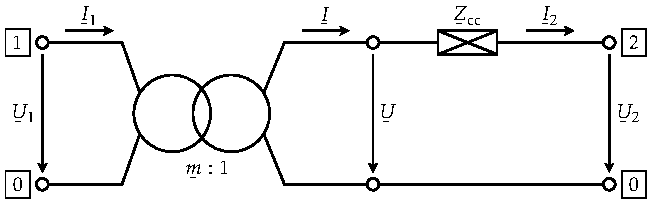
\includegraphics{Imatges/Cap-FluxCarregues-Trafo.pdf}
\caption{Circuit equivalent d'un transformador amb regulaci\'{o}
variable i decalatge} \label{pic:equiv_trafo_reg_decal}
\end{figure}

En l'esquema anterior, $\cmplx{Z}\ped{cc}$ \'{e}s la imped\`{a}ncia de curt
circuit per fase del transformador, i $\cmplx{m} : 1$ \'{e}s la seva
relaci\'{o} de transformaci\'{o}. El par\`{a}metre $\cmplx{m}$ \'{e}s un valor
complex, ja que el transformador a m\'{e}s de variar el m\`{o}dul de la
tensi\'{o}, tamb\'{e} varia  el seu argument; les tensions prim\`{a}ria i
secund\`{a}ria tenen, per tant,  diferent m\`{o}dul i un decalatge entre els
seus arguments.

Si la imped\`{a}ncia es volgu\'{e}s representar en el primari del
transformador, el seu valor seria $|\cmplx{m}|^2 \cmplx{Z}\ped{cc}$.

En el circuit de la Figura \vref{pic:equiv_trafo_reg_decal} es
compleix: \index{transformadors amb regulaci\'{o} variable i
decalatge!equacions de funcionament}
\begin{equation}
   \cmplx{U}_1 = \cmplx{m} \,\cmplx{U} = \cmplx{m}\,
   [\cmplx{U}_2+\cmplx{Z}\ped{cc}\cmplx{I}_2]
   \qquad\qquad
   \cmplx{I}_1 = \frac{\cmplx{I}}{\cmplx{m}^*} = \frac{\cmplx{I}_2}{\cmplx{m}^*}
   \qquad\qquad
   \cmplx{U}_1 \cmplx{I}_1^* = \cmplx{U} \,\cmplx{I}^*
\end{equation}

Utilitzant aquestes tres equacions, podem escriure:
\begin{equation}
   \cmplx{I}_1 = \frac{\cmplx{U}_1}{|\cmplx{m}|^2 \cmplx{Z}\ped{cc}} - \frac{\cmplx{U}_2}
   {\cmplx{m}^* \cmplx{Z}\ped{cc}} \qquad\qquad
   - \cmplx{I}_2 = - \frac{\cmplx{U}_1}{\cmplx{m} \,\cmplx{Z}\ped{cc}} + \frac{\cmplx{U}_2}
   {\cmplx{Z}\ped{cc}}
\end{equation}

Aquestes equacions ens permeten escriure, directament, la
contribuci\'{o} d'un transformador amb regulaci\'{o} variable i decalatge, a
la matriu d'admit\`{a}ncies de nus $\mcmplx{Y}\ped{N}$ de la xarxa a la
qual pertany: \index{transformadors amb regulaci\'{o} variable i
decalatge!matriu d'admit\`{a}ncies de nus $\mcmplx{Y}\ped{N}$}
\index{matriu!d'admit\`{a}ncies de nus $\mcmplx{Y}\ped{N}$}
\begin{equation} \label{eq:yn_trafo_reg_decal}
   \mcmplx{Y}\ped{N} = \begin{pmatrix}
     \dfrac{1}{|\cmplx{m}|^2 \cmplx{Z}\ped{cc}} & - \dfrac{1}
   {\cmplx{m}^* \cmplx{Z}\ped{cc}} \\[2.5ex]
     - \dfrac{1}{\cmplx{m} \,\cmplx{Z}\ped{cc}} & \dfrac{1}
   {\cmplx{Z}\ped{cc}}
   \end{pmatrix}
\end{equation}

Com es pot veure, $\mcmplx{Y}\ped{N}(1,2) \neq
\mcmplx{Y}\ped{N}(2,1)$; aix\`{o} ens indica que no existeix un esquema
equivalent en {"<}$\piup${">} del transformador, format tan sols per
elements passius.

Els fluxos de pot\`{e}ncia a trav\'{e}s del transformador, $\cmplx{S}_{12}$
(del nus 1 al 2), i $\cmplx{S}_{21}$ (del nus 2 a l'1), v\'{e}nen donats
per les expressions: \index{transformadors amb regulaci\'{o} variable i
decalatge!fluxos de pot\`{e}ncia}
\begin{alignat}{2}
   \cmplx{S}_{12} &= \cmplx{U}_1 \left[ \frac{\cmplx{U}_1}{|\cmplx{m}|^2 \cmplx{Z}\ped{cc}} - \frac{\cmplx{U}_2}{\cmplx{m}^* \cmplx{Z}\ped{cc}} \right]^* &&= \frac{\cmplx{U}_1}{\cmplx{m}\, \cmplx{Z}\ped{cc}^*} \left[ \frac{\cmplx{U}_1}{\cmplx{m}} - \cmplx{U}_2 \right]^* \label{eq:s12_trafo_reg_decal} \\[1.5ex]
   \cmplx{S}_{21} &= \cmplx{U}_2 \left[ - \frac{\cmplx{U}_1}{\cmplx{m} \,\cmplx{Z}\ped{cc}} + \frac{\cmplx{U}_2} {\cmplx{Z}\ped{cc}} \right]^* &&= \frac{\cmplx{U}_2}{\cmplx{Z}\ped{cc}^*} \left[  \cmplx{U}_2 - \frac{\cmplx{U}_1}{\cmplx{m}}  \right]^* \label{eq:s21_trafo_reg_decal}
\end{alignat}

Finalment, les p\`{e}rdues de transmissi\'{o} del transformador
$\Delta\cmplx{S}$, v\'{e}nen donades per l'expressi\'{o}:
\index{transformadors amb regulaci\'{o} variable i decalatge!p\`{e}rdues de
transmissi\'{o}}
\begin{equation} \label{eq:ds_trafo_reg_decal}
   \Delta\cmplx{S} = \cmplx{S}_{12} + \cmplx{S}_{21} = \frac{1}{\cmplx{Z}\ped{cc}^*}  \left|
    \frac{\cmplx{U}_1}{\cmplx{m}} - \cmplx{U}_2 \right|^2
\end{equation}


\subsection{Transformadors amb regulaci\'{o} variable sense decalatge} \label{sec:trafo_reg}
\index{transformadors amb regulaci\'{o} variable sense decalatge}

Aquest \'{e}s un cas particular de l'anterior, on el transformador no
origina decalatge de fase entre les tensions prim\`{a}ria i secund\`{a}ria.
En aquest cas, la relaci\'{o} de transformaci\'{o} $m : 1$ \'{e}s un valor real.

A partir de l'equaci\'{o}  \eqref{eq:yn_trafo_reg_decal}, substituint
$\cmplx{m}$ per $m$, obtenim la contribuci\'{o} d'un transformador amb
regulaci\'{o} variable sense decalatge, a la matriu d'admit\`{a}ncies de nus
$\mcmplx{Y}\ped{N}$ de la xarxa a la qual pertany:
\index{transformadors amb regulaci\'{o} variable sense decalatge!matriu
d'admit\`{a}ncies de nus $\mcmplx{Y}\ped{N}$}
\index{matriu!d'admit\`{a}ncies de nus $\mcmplx{Y}\ped{N}$}
\begin{equation}
   \mcmplx{Y}\ped{N} = \begin{pmatrix}
     \dfrac{1}{m^2 \cmplx{Z}\ped{cc}} & - \dfrac{1}{m \,\cmplx{Z}\ped{cc}} \\[2.5ex]
     - \dfrac{1}{m \,\cmplx{Z}\ped{cc}} & \dfrac{1}{\cmplx{Z}\ped{cc}}
   \end{pmatrix}
\end{equation}

An\`{a}logament, podem obtenir els fluxos de pot\`{e}ncia a trav\'{e}s del
transformador, $\cmplx{S}_{12}$ (del nus 1 al 2), i $\cmplx{S}_{21}$
(del nus 2 a l'1), i les seves p\`{e}rdues de transmissi\'{o}
$\Delta\cmplx{S}$, a partir de les equacions
\eqref{eq:s12_trafo_reg_decal},  \eqref{eq:s21_trafo_reg_decal} i
\eqref{eq:ds_trafo_reg_decal}: \index{transformadors amb regulaci\'{o}
variable sense decalatge!fluxos de pot\`{e}ncia} \index{transformadors
amb regulaci\'{o} variable sense decalatge!p\`{e}rdues de transmissi\'{o}}
\begin{align}
   \cmplx{S}_{12} &= \cmplx{U}_1 \left[ \frac{\cmplx{U}_1}{m^2 \cmplx{Z}\ped{cc}} - \frac{\cmplx{U}_2}{m \cmplx{Z}\ped{cc}} \right]^* = \frac{\cmplx{U}_1}{m \,\cmplx{Z}\ped{cc}^*} \left[ \frac{\cmplx{U}_1}{m} - \cmplx{U}_2 \right]^*  \\[1.5ex]
   \cmplx{S}_{21} &= \cmplx{U}_2 \left[ - \frac{\cmplx{U}_1}{m \,\cmplx{Z}\ped{cc}} + \frac{\cmplx{U}_2} {\cmplx{Z}\ped{cc}} \right]^* = \frac{\cmplx{U}_2}{\cmplx{Z}\ped{cc}^*} \left[  \cmplx{U}_2 - \frac{\cmplx{U}_1}{m}  \right]^* \\[1.5ex]
 \Delta\cmplx{S} &= \cmplx{S}_{12} + \cmplx{S}_{21} = \frac{1}{\cmplx{Z}\ped{cc}^*}  \left|
    \frac{\cmplx{U}_1}{m} - \cmplx{U}_2 \right|^2
\end{align}


El circuit equivalent d'aquest tipus de transformador, tamb\'{e} \'{e}s el de la
 Figura \vref{pic:equiv_trafo_reg_decal}, substituint $\cmplx{m}:1$ per $m:1$; no
 obstant, at\`{e}s que en aquest cas es compleix $\mcmplx{Y}\ped{N}(1,2) = \mcmplx{Y}\ped{N}(2,1)$, tamb\'{e}
 existeix un circuit equivalent en {"<}$\piup${">}, format per una imped\`{a}ncia longitudinal i dues admit\`{a}ncies transversals, tal com es pot veure en la Figura  \vref{pic:equiv_trafo_reg}.
\index{transformadors amb regulaci\'{o} variable sense decalatge!circuit
equivalent en \guillemotleft$\piup$\guillemotright}
\begin{figure}[htb]
\vspace{-1mm}\centering
    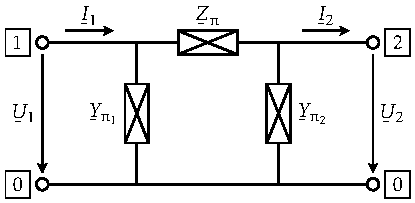
\includegraphics{Imatges/Cap-FluxCarregues-Trafo-Pi.pdf}
\caption{Circuit equivalent d'un transformaci\'{o} amb regulaci\'{o}
variable sense decalatge} \label{pic:equiv_trafo_reg}
\end{figure}

Els valors dels par\`{a}metres d'aquest circuit equivalent s\'{o}n:
\begin{align}
   \cmplx{Z}_\piup &= m \, \cmplx{Z}\ped{cc} \\[1.5ex]
   \cmplx{Y}_{\piup_1} &= \frac{1-m}{m^2 \,\cmplx{Z}\ped{cc}} \\[1.5ex]
   \cmplx{Y}_{\piup_2} &= \frac{m-1}{m\, \cmplx{Z}\ped{cc}}
\end{align}

\section{Tipus de nusos} \index{flux de c\`{a}rregues!tipus de nusos}

Cadascun dels nusos d'un sistema el\`{e}ctric de pot\`{e}ncia, t\'{e} quatre
magnituds associades: les potencies activa i reactiva injectades des
de l'exterior de la xarxa, i el m\`{o}dul i l'argument de la seva
tensi\'{o}.

Usualment, en cada nus del sistema es coneixen dues de les quatre
magnituds anteriors; segons quines siguin aquestes magnituds, es
poden distingir els seg\"{u}ents tipus de nusos:
\begin{dinglist}{'167}
    \item \textbf{Nus de potencial zero}. El terra \'{e}s sempre el nus de refer\`{e}ncia, o de potencial zero, de la
    xarxa, i per tant, totes les tensions de la xarxa hi s\'{o}n referides.
    Al terra s'assigna el n\'{u}mero de nus 0, i per tant no forma part de la matriu d'admit\`{a}ncies de nus de la xarxa.
\index{nus!de potencial zero}\index{nus!de refer\`{e}ncia}

   \item \textbf{Nus flotant}. \'{E}s un nus on es mant\'{e} constant la tensi\'{o} en m\`{o}dul i argument,
   essent inc\`{o}gnites les pot\`{e}ncies activa i reactiva injectades a la xarxa des de l'exterior.
    Generalment, acostuma a ser el nus que m\'{e}s s'aproxima a un nus de pot\`{e}ncia infinita. Des del
    punt de vista de la xarxa, correspon clarament a un generador ideal de tensi\'{o}.
    \index{nus!flotant}

Tan sols hi pot haver un nus d'aquest tipus en tota la xarxa.
   \item \textbf{Nus de tensi\'{o} controlada}. En aquest nus es coneix el m\`{o}dul de la tensi\'{o} i la
   pot\`{e}ncia activa injectada a la xarxa des de l'exterior, essent inc\`{o}gnites l'argument de la tensi\'{o} i la pot\`{e}ncia
   reactiva injectada des de l'exterior. En aquests nusos, sovint s'imposen l\'{\i}mits a la pot\`{e}ncia reactiva.
\index{nus!de tensi\'{o} controlada}

   \item \textbf{Nus de c\`{a}rrega}. En aquest nus es coneixen les pot\`{e}ncies activa i reactiva
   injectades a la xarxa des de l'exterior, i s\'{o}n inc\`{o}gnites el m\`{o}dul i l'argument de la tensi\'{o}.
   Aquests nusos poden ser tant de consum com de generaci\'{o}.
   \index{nus!de c\`{a}rrega}

En els nusos on incideix un transformador amb relaci\'{o} de
transformaci\'{o} variable sense decalatge, hi pot haver tres magnituds
conegudes: les pot\`{e}ncies activa i reactiva injectades i el m\`{o}dul de
la tensi\'{o}, el qual es vol mantenir constant mitjan\c{c}ant l'ajust de la
relaci\'{o} de transformaci\'{o}; les inc\`{o}gnites s\'{o}n per tant, l'argument de
la tensi\'{o} i la citada relaci\'{o} de transformaci\'{o} del transformador.
\end{dinglist}

En la Taula \vref{taula:tipus_nusos} es resumeix el que s'ha exposat
sobre els diferents tipus de nusos en un sistema el\`{e}ctric de
pot\`{e}ncia.
\begin{table}[htb]
   \caption{\label{taula:tipus_nusos} Tipus de nusos en un sistema el\`{e}ctric de pot\`{e}ncia}
   \begin{center}\begin{tabular}{lccccc}
   \toprule[1pt]
   \multirow{2}{15mm}{\rule{0mm}{4.5mm}Tipus\\de nus}  & \multicolumn{2}{c}{Tensi\'{o}} &
   \multicolumn{2}{c}{Pot\`{e}ncia injectada} & \renewcommand*{\multirowsetup}{\centering}
   \multirow{2}{25mm}{\rule{0mm}{4.5mm}Relaci\'{o} de\\transformaci\'{o}} \\
   \cmidrule(rl){2-3} \cmidrule(rl){4-5}
    & m\`{o}dul & argument & activa & reactiva &  \\
   \midrule
   Flotant                &  \textcolor{Green}{\ding{51}} & \textcolor{Green}{\ding{51}} & \textcolor{Red}{\ding{55}} & \textcolor{Red}{\ding{55}} & --- \\
   De tensi\'{o} controlada   &  \textcolor{Green}{\ding{51}} & \textcolor{Red}{\ding{55}} & \textcolor{Green}{\ding{51}} & \textcolor{Red}{\ding{55}} & --- \\
   De c\`{a}rrega (sense trafo)             &  \textcolor{Red}{\ding{55}} & \textcolor{Red}{\ding{55}} & \textcolor{Green}{\ding{51}} & \textcolor{Green}{\ding{51}} & --- \\
   De c\`{a}rrega (amb trafo) &  \textcolor{Green}{\ding{51}} & \textcolor{Red}{\ding{55}} & \textcolor{Green}{\ding{51}} & \textcolor{Green}{\ding{51}} & \textcolor{Red}{\ding{55}} \\

   \midrule
   \multicolumn{6}{c}{\textcolor{Green}{\ding{51}} valor conegut \hspace{6ex} \textcolor{Red}{\ding{55}} valor inc\`{o}gnita
   \hspace{6ex} --- no aplicable} \\
   \bottomrule[1pt]
   \end{tabular} \end{center}
\end{table}


\section{Formulaci\'{o} del problema}\label{sec:formul_prob} \index{flux de c\`{a}rregues!formulaci\'{o} del problema}

Comencem per considerar una xarxa el\`{e}ctrica amb els nusos numerats
$1,\ldots,n$, i essent el terra el nus 0 de refer\`{e}ncia; una de les
maneres de descriure aquesta xarxa \'{e}s utilitzant el m\`{e}tode dels
nusos, descrit en el Cap\'{\i}tol \ref{chap:nusos}:
\begin{equation}
    \mcmplx{Y}\ped{N} \mcmplx{V}\ped{N} = \mcmplx{J}\ped{N}
\end{equation}

Tenint en compte que els elements de $\mcmplx{J}\ped{N}$,
$\mcmplx{V}\ped{N}$ i $\mcmplx{Y}\ped{N}$ s\'{o}n $\cmplx{j}_i$,
$\cmplx{v}_i$ i  $\cmplx{y}_{ik}$ ($i,k=1,\ldots,n$) respectivament,
i que aquests valors, suposem que estan expressats en p.u. (vegeu la
Secci\'{o} \ref{sec:seccio_pu}), l'equaci\'{o} anterior queda expressada de
la seg\"{u}ent manera:
\begin{equation}
    \sum^n_{k=1}\, \cmplx{y}_{ik} \cmplx{v}_k = \cmplx{j}_i \qquad\qquad i=1,\ldots,n
\end{equation}

En cadascun dels nusos de la xarxa es compleix la seg\"{u}ent relaci\'{o}
per a la pot\`{e}ncia complexa $\cmplx{s}_i = p_i + \ju q_i$, injectada
al nus des de l'exterior:
\begin{equation}
    \cmplx{s}_i^* = p_i - \ju q_i = \cmplx{v}_i^* \cmplx{j}_i = \cmplx{v}_i^*
    \sum^n_{k=1}\, \cmplx{y}_{ik} \cmplx{v}_k \qquad\qquad i=1,\ldots,n \label{eq:sconj}
\end{equation}

Ara b\'{e}, si expressem els potencials $\cmplx{v}_i$ a partir dels seus m\`{o}duls $|\cmplx{v}_i|$
i arguments $\delta_i$, i les admit\`{a}ncies $\cmplx{y}_{ik}$ a partir de les seves parts
reals $g_{ik}$ i imagin\`{a}ries $b_{ik}$, tenim:
\begin{align}
    \cmplx{v}_i &=|\cmplx{v}_i| \eu^{\ju\delta_i} = |\cmplx{v}_i|
    (\cos\delta_i+\ju\sin\delta_i) & i & =1,\ldots,n\\
    \cmplx{y}_{ik} &= g_{ik} + \ju b_{ik} & i,k & =1,\ldots,n \\
    p_i - \ju q_i &= |\cmplx{v}_i| (\cos\delta_i - \ju\sin\delta_i) \sum^n_{k=1} (g_{ik} + \ju
    b_{ik}) |\cmplx{v}_k| (\cos\delta_k + \ju\sin\delta_k) & i & =1,\ldots,n
\end{align}

Finalment, si separem la darrera equaci\'{o} en dues, una per a  la part real i  una altra per
a la part imagin\`{a}ria, tenim:
\begin{align}
    p_i - |\cmplx{v}_i| \sum^n_{k=1}  |\cmplx{v}_k| \bigl[ g_{ik} \cos(\delta_k - \delta_i) -
     b_{ik} \sin(\delta_k - \delta_i) \bigr] &= 0  & i&=1,\ldots,n\label{eq:p0} \\
    q_i + |\cmplx{v}_i| \sum^n_{k=1}  |\cmplx{v}_k| \bigl[ g_{ik} \sin(\delta_k - \delta_i) +
      b_{ik} \cos(\delta_k - \delta_i) \bigr] &= 0 & i&=1,\ldots,n\label{eq:q0}
\end{align}

Resolent de forma simult\`{a}nia les equacions \eqref{eq:p0} i
\eqref{eq:q0}, trobar\'{\i}em els potencials dels nusos de la xarxa
respecte al terra, i posteriorment, utilitzant l'equaci\'{o}
\eqref{eq:sconj}, obtindr\'{\i}em la pot\`{e}ncia injectada en cada nus des
de l'exterior. Ara b\'{e}, \'{e}s clar que no es poden plantejar les
equacions \eqref{eq:p0} i \eqref{eq:q0} en tots els nusos de la
xarxa, ja que en alguns d'ells els valors $p_i$ o $q_i$ s\'{o}n
desconeguts (vegeu la Taula \vref{taula:tipus_nusos}). Per tant, per
tal de resoldre el problema del flux de c\`{a}rregues en un sistema
el\`{e}ctric de pot\`{e}ncia, cal seguir els passos seg\"{u}ents:
\begin{dingautolist}{'312}
    \item Es numeren tots els nusos de la xarxa, comen\c{c}ant pel n\'{u}mero 1. El terra \'{e}s sempre el nus 0 de refer\`{e}ncia.
   \item Es forma la matriu d'admit\`{a}ncies de nusos $\mcmplx{Y}\ped{N}$, tal com s'ha
   explicat en el Cap\'{\i}tol \ref{chap:nusos}.
   \item Es forma l'equaci\'{o} \eqref{eq:p0} per a tots els nusos de tensi\'{o} controlada i per
   a tots els nusos de c\`{a}rrega. Cal tenir en compte que la pot\`{e}ncia activa  injectada $p_i$ es considera
   positiva quan entra des de l'exterior a la xarxa, i negativa en cas contrari.
   \item Es forma l'equaci\'{o} \eqref{eq:q0} per a tots els nusos de c\`{a}rrega. Cal tenir en compte
   que la pot\`{e}ncia reactiva injectada $q_i$  es considera positiva quan entra des de l'exterior a la xarxa, i negativa en cas contrari.
   \item Es resol de forma num\`{e}rica el sistema d'equacions no lineals, format en els dos
   passos anteriors; com a valors inicials de les inc\`{o}gnites, es poden prendre els valors
   seg\"{u}ents:
   \begin{dinglist}{'167}
    \item M\`{o}duls dels potencials: m\`{o}dul del potencial del nus flotant
    \item Arguments dels potencials: argument del potencial del nus flotant
    \item Relacions de transformaci\'{o}: 1
   \end{dinglist}
   \item Si \'{e}s necessari,  es pot calcular la pot\`{e}ncia injectada en els nusos de la xarxa
   des de l'exterior, en aquells nusos on no es
   coneix aquest valor, utilitzant    l'equaci\'{o} \eqref{eq:sconj}.
\end{dingautolist}

\begin{exemple}
Es tracta de trobar en la xarxa seg\"{u}ent, els potencials dels nusos 2
i 3, i les pot\`{e}ncies subministrades pels generador dels nusos 1 i 2;
tots els valors estan donats en p.u.
\begin{figure}[htb]
\centering
    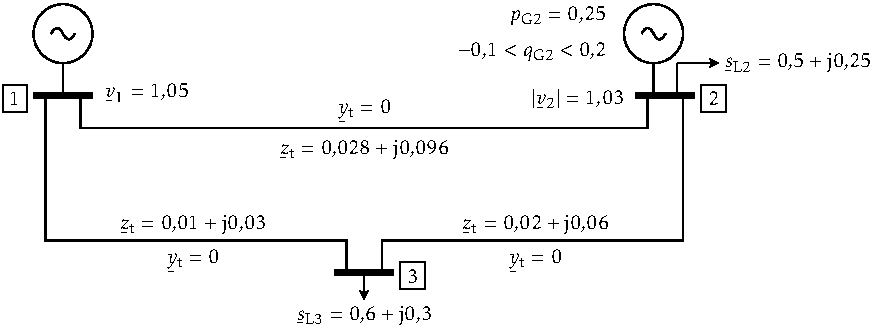
\includegraphics{Imatges/Cap-FluxCarregues-Exemple1.pdf}
\end{figure}

Comencem formant la matriu d'admit\`{a}ncies de nus:
\begin{align*}
\mcmplx{Y}\ped{N} &= \begin{pmatrix}
\frac{1}{0{,}028+\ju0{,}096} + \frac{1}{0{,}01+\ju0{,}03} & -\frac{1}{0{,}028+\ju0{,}096}  &  -\frac{1}{0{,}01+\ju0{,}03}\\
-\frac{1}{0{,}028+\ju0{,}096} & \frac{1}{0{,}028+\ju0{,}096} + \frac{1}{0{,}02+\ju0{,}06} &  -\frac{1}{0{,}02+\ju0{,}06}\\
-\frac{1}{0{,}01+\ju0{,}03} & -\frac{1}{0{,}02+\ju0{,}06} &
\frac{1}{0{,}01+\ju0{,}03} + \frac{1}{0{,}02+\ju0{,}06}
\end{pmatrix} = \\[1.5ex]
 &= \begin{pmatrix}
12{,}8 - \ju 39{,}6 & -2{,}8 + \ju 9{,}6 & -10{,}0 + \ju 30{,}0 \\
-2{,}8 + \ju 9{,}6 & 7{,}8 - \ju 24{,}6 & -5{,}0 + \ju 15{,}0 \\
-10{,}0 + \ju 30{,}0 & -5{,}0 + \ju 15{,}0 & 15{,}0 - \ju 45{,}0
\end{pmatrix}
\end{align*}

El nus 1 \'{e}s el nus flotant, el nus 2 en un nus de tensi\'{o} controlada
i el nus 3 \'{e}s un nus de c\`{a}rrega; formarem, per tant, l'equaci\'{o}
\eqref{eq:p0} pels nusos 2 i 3, i l'equaci\'{o} \eqref{eq:q0} pel nus 3:
\begin{align*}
\begin{split}
0{,}25-0{,}5 &- 1{,}03\cdot \bigl( 1{,}05\cdot [-2{,}8
\cdot\cos(-\delta_2) - 9{,}6
\cdot\sin( -\delta_2)]  + 1{,}03 \cdot 7{,}8 {}+ \\
&+ |\cmplx{v}_3|\cdot [-5{,}0 \cdot\cos(\delta_3-\delta_2) -
15{,}0\cdot \sin(\delta_3-\delta_2)]
 \bigr)  = 0 \end{split} \\[1.5ex]
\begin{split}
-0{,}6 &- |\cmplx{v}_3| \cdot \bigl( 1{,}05\cdot [-10{,}0
\cdot\cos(-\delta_3)
- 30{,}0\cdot\sin(-\delta_3)]  + \\
&+ 1{,}03\cdot [-5{,}0\cdot\cos(\delta_2-\delta_3) -
15{,}0\cdot\sin(\delta_2-\delta_3)]
 + |\cmplx{v}_3| \cdot15{,}0 \bigr)  = 0 \end{split}  \\[1.5ex]
\begin{split}
-0{,}3 &+ |\cmplx{v}_3|\cdot \bigl( 1{,}05
\cdot[-10{,}0\cdot\sin(-\delta_3) +
30{,}0\cdot\cos(-\delta_3)]  + \\
&+ 1{,}03 \cdot[-5{,}0\cdot\sin(\delta_2-\delta_3) +
15{,}0\cdot\cos(\delta_2-\delta_3)] + |\cmplx{v}_3|\cdot (-45{,}0)
\bigr)  = 0 \end{split}
\end{align*}

Resolent aquest sistema d'equacions no lineals, amb els valors
inicials $|\cmplx{v}_3|=1{,}05$ i $\delta_2=\delta_3=0$, obtenim:
\begin{gather*}
   \delta_2=-0{,}015277\unit{rad} \\[1ex]
   |\cmplx{v}_3|=1{,}033587 \qquad \delta_3=-0{,}014301\unit{rad}
\end{gather*}

Calcularem a continuaci\'{o}, les pot\`{e}ncies injectades en els nusos 1 i
2, utilitzant l'equaci\'{o} \eqref{eq:sconj}:
\begin{align*}
\begin{split}
\cmplx{s}_1^* &= 1{,}05 \cdot\bigl[ (12{,}8-\ju39{,}6) \cdot 1{,}05
+
(-2{,}8+\ju9{,}6) \cdot 1{,}03\cdot\eu^{-\ju0{,}015277} + \\
&+ (-10{,}0+\ju30{,}0) \cdot 1{,}033587\cdot\eu^{-\ju0{,}014301}
\bigr] = 0{,}85680 - \ju 0{,}52169
\end{split} \\[1.5ex]
\cmplx{s}_1 &= 0{,}85680 + \ju 0{,}52169 \\[1.5ex]
\begin{split}
\cmplx{s}_2^* &= 1{,}03 \cdot\eu^{\ju0{,}015277} \cdot\bigl[
(-2{,}8+\ju9{,}6) \cdot 1{,}05 +
 (7{,}8-\ju24{,}6) \cdot 1{,}03\cdot\eu^{-\ju0{,}015277} + \\
& + (-5{,}0+\ju15{,}0) \cdot 1{,}033587\cdot\eu^{-\ju0{,}014301}
\bigr] = -0{,}25000 + \ju 0{,}20050
\end{split} \\[1.5ex]
 \cmplx{s}_2 &= -0{,}25000 - \ju 0{,}20050
\end{align*}

Per tant, les pot\`{e}ncies subministrades a la xarxa pels generadors
dels nusos 1 i 2, s\'{o}n:
\begin{align*}
\cmplx{s}\ped{G1} &= \cmplx{s}_1 = 0{,}85680 + \ju 0{,}52169 \\[1ex]
\cmplx{s}\ped{G2} &= \cmplx{s}\ped{L2} + \cmplx{s}_2 = 0{,}5 + \ju
0{,}25 -0{,}25000 - \ju 0{,}20050  = 0{,}25000 + \ju 0{,}04950
\end{align*}

El valor calculat de la pot\`{e}ncia activa subministrada pel generador
del nus 2, es
 correspon, evidentment, amb el valor que s'ha utilitzat com a dada per
resoldre la xarxa ($p\ped{G2}=0{,}25$).

Pel que fa a la potencia reactiva subministrada pel generador del
nus 2, s'observa que es troba dins dels  marges especificats
($-0{,}1<q\ped{G2}<0{,}2$).
\end{exemple}

\begin{exemple}

Es tracta de trobar en la xarxa seg\"{u}ent, el potencial del nus 2 i la
pot\`{e}ncia subministrada pel generador del nus 1; tots els valors
estan donats en p.u. Es consideren dos casos:
\begin{enumerate}
   \renewcommand{\labelenumi}{\alph{enumi})}
   \item La bateria de condensadors del nus 2 est\`{a} desconnectada.
   \item Es connecta la bateria de condensadors del nus 2, per tal de mantenir el m\`{o}dul de
   la tensi\'{o} d'aquest nus al valor $|\cmplx{v}_2|=1{,}03$.
\end{enumerate}
\begin{figure}[htb]
\centering
    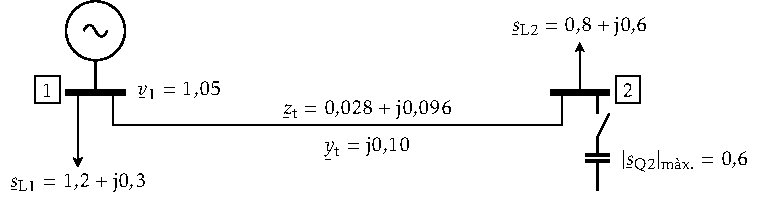
\includegraphics{Imatges/Cap-FluxCarregues-Exemple2.pdf}
\end{figure}

Comencem formant la matriu d'admit\`{a}ncies de nus:
\[
\mcmplx{Y}\ped{N} = \begin{pmatrix}
  \frac{\ju 0{,}10}{2} + \frac{1}{0{,}028+\ju0{,}096} & -\frac{1}{0{,}028+\ju0{,}096} \\
  -\frac{1}{0{,}028+\ju0{,}096} & \frac{\ju 0{,}10}{2} + \frac{1}{0{,}028+\ju0{,}096} \\
\end{pmatrix} =
\begin{pmatrix}
  2{,}80 -\ju9{,}55 & -2{,}80 +\ju9{,}60 \\
  -2{,}80 +\ju9{,}60 & 2{,}80 -\ju9{,}55 \\
\end{pmatrix}
\]

a) En aquest cas, el nus 1 \'{e}s el nus flotant, i el nus 2 en un nus
de c\`{a}rrega.

Formem a continuaci\'{o} les equacions \eqref{eq:p0} i \eqref{eq:q0} pel
nus 2:
\begin{align*}
-0{,}8 - |\cmplx{v}_2| \cdot \bigl( 1{,}05\cdot [-2{,}80\cdot \cos(-\delta_2) - 9{,}60 \cdot
\sin( -\delta_2)]  + |\cmplx{v}_2| \cdot 2{,}80 \bigr) &= 0 \\
-0{,}6 + |\cmplx{v}_2| \cdot\bigl( 1{,}05 \cdot[-2{,}80\cdot\sin(-\delta_2) +
9{,}60\cdot\cos( -\delta_2)]  + |\cmplx{v}_2|\cdot (-9{,}55) \bigr) &= 0
\end{align*}

Resolent aquest sistema d'equacions no lineals, amb els valors inicials $|\cmplx{v}_2|=1{,}05$ i $\delta_2=0$, obtenim:
\[ |\cmplx{v}_2|=0{,}970306 \qquad \delta_2=-0{,}060222\unit{rad} \]

Calculem a continuaci\'{o} la pot\`{e}ncia que circula des del nus 1 cap al
nus 2, utilitzant l'equaci\'{o} \eqref{eq:lin_s12}:
\[
\cmplx{s}_{12} = 1{,}05\cdot \left[ \frac{\ju0{,}10}{2} \cdot1{,}05 + \frac{ 1{,}05 -
0{,}970306\cdot\eu^{-\ju0{,}060222}} {0{,}028+\ju0{,}096} \right]^* = 0{,}82813 + \ju
0{,}59423
\]

Per tant, la pot\`{e}ncia subministrada a la xarxa pel generador del nus
1, \'{e}s:
\[ \cmplx{s}\ped{G1} = \cmplx{s}\ped{L1} + \cmplx{s}_{12} = 1{,}2+\ju0{,}3 + 0{,}82812 + \ju 0{,}59423 = 2{,}02813 + \ju 0{,}89423 \]

b) En aquest cas, el nus 1 \'{e}s el nus flotant, i el nus 2 en un nus
de tensi\'{o} controlada.

Formem a continuaci\'{o} l'equaci\'{o} \eqref{eq:p0} pel nus 2:
\[
-0{,}8 - 1{,}03\cdot \bigl( 1{,}05\cdot [-2{,}80\cdot\cos(-\delta_2) - 9{,}60\cdot\sin(
-\delta_2)] + 1{,}03\cdot 2{,}80 \bigr) = 0
\]

Resolent aquesta equaci\'{o} no lineal, amb el valor inicial $\delta_2=0$, obtenim:
\[\delta_2=-0{,}072323\unit{rad}\]

Calculem a continuaci\'{o} la pot\`{e}ncia que circula entre els nusos 1 i
2, utilitzant les equacions \eqref{eq:lin_s12} i \eqref{eq:lin_s21}:
\begin{align*}
\cmplx{s}_{12} &= 1{,}05 \cdot\left[ \frac{\ju0{,}10}{2} \cdot1{,}05 + \frac{ 1{,}05 -
1{,}03\cdot\eu^{-\ju0{,}072323}} {0{,}028+\ju0{,}096} \right]^* =
0{,}81695 - \ju 0{,}04520 \\[1.5ex]
\cmplx{s}_{21} &= 1{,}03\cdot \eu^{-\ju0{,}072323} \cdot\left[ \frac{\ju0{,}10}{2}\cdot
1{,}03\cdot \eu^{-\ju0{,}072323} + \frac{ 1{,}03\cdot\eu^{-\ju0{,}072323} -1{,}05}
{0{,}028+\ju0{,}096} \right]^* = -0{,}80000 - \ju 0{,}00484
\end{align*}

Per tant, les pot\`{e}ncies subministrades a la xarxa pel generador del
nus 1 i pel condensador del nus 2, s\'{o}n:
\begin{align*}
 \cmplx{s}\ped{G1} &= \cmplx{s}\ped{L1} + \cmplx{s}_{12} = 1{,}2+\ju0{,}3 + 0{,}81695 - \ju 0{,}04520 = 2{,}01695 + \ju 0{,}25480 \\
 \cmplx{s}\ped{Q2} &= \cmplx{s}\ped{L2} + \cmplx{s}_{21} = 0{,}8+\ju0{,}6 - 0{,}80000 - \ju 0{,}00484 =  \ju 0{,}59516
\end{align*}

S'ha calculat el valor de $\cmplx{s}\ped{Q2}$, per tal de comprovar
que est\`{a} dins dels marges especificats
($|\cmplx{s}\ped{Q2}|_{\text{m\`{a}x.}}=0{,}6$); si aix\`{o} no fos aix\'{\i},
caldria fixar $\cmplx{s}\ped{Q2}$ al seu valor m\`{a}xim i tornar a
recalcular la xarxa, passant el nus 2 a ser un nus de c\`{a}rrega, i
essent, per tant, desconeguda la seva tensi\'{o}.
\end{exemple}

\break
\begin{exemple}
En el sistema de la figura seg\"{u}ent, es vol mantenir el m\`{o}dul del
potencial del nus 2 fixat al valor indicat, mitjan\c{c}ant l'ajust
adequat de la relaci\'{o} de transformaci\'{o} del transformador connectat
entre els nusos 1 i 2. Es tracta per tant de trobar aquest valor,
aix\'{\i} com el potencial del nus 2; tots els valors estan donats en
p.u.

\begin{figure}[h!]
\centering
    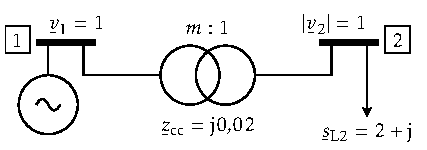
\includegraphics{Imatges/Cap-FluxCarregues-Exemple3.pdf}
\end{figure}

Comencem formant la matriu d'admit\`{a}ncies de nus:
\[
\mcmplx{Y}\ped{N} = \begin{pmatrix}
\dfrac{1}{\ju0{,}02 \,m^2}  &  -\dfrac{1}{\ju0{,}02 \,m} \\[1.5ex]
-\dfrac{1}{\ju0{,}02\, m}   & \dfrac{1}{\ju0{,}02}
\end{pmatrix} =
\begin{pmatrix}
-\ju\dfrac{50}{m^2}  &  \ju\dfrac{50}{m} \\[1.5ex]
\ju\dfrac{50}{m}     & -\ju 50
\end{pmatrix}
\]

El nus 1 \'{e}s el nus flotant i el nus 2 en un nus de c\`{a}rrega;
formarem, per tant,  les equacions \eqref{eq:p0} i \eqref{eq:q0} pel
nus 2:
\begin{align*}
-2 - 1 \cdot\left( 1 \cdot\left[ 0 -\frac{50}{m} \cdot\sin(-\delta_2) \right]  + 0 \right)  = 0   \\[1.5ex]
-1 + 1 \cdot\left( 1 \cdot\left[0 + \frac{50}{m}
\cdot\cos(-\delta_2) \right]  + 1\cdot (-50) \right)  = 0
\end{align*}

Resolent aquest sistema d'equacions no lineals, amb els valors
inicials $\delta_2=0$ i $m=1$, obtenim:
\begin{align*}
   \delta_2 &= -0{,}039196\unit{rad} \\[1ex]
   m & =0{,}979639
\end{align*}

En un cas real, el par\`{a}metre $m$ del transformador \'{u}nicament podria
prendre uns quants valors discrets; caldria doncs assignar a $m$ el
valor m\'{e}s pr\`{o}xim al calculat, escollint entre els diversos valors
possibles, i tornar a recalcular la xarxa, passant la tensi\'{o} del nus
2 a ser un valor desconegut.

\end{exemple}

\section{Control del flux de pot\`{e}ncia} \index{flux de c\`{a}rregues!control del flux de
pot\`{e}ncia}\label{sec:control-flux-pot}

Veurem breument a continuaci\'{o}, les diverses formes que existeixen
per controlar el flux de pot\`{e}ncia activa i reactiva en les branques
d'una xarxa, aix\'{\i} com els m\`{e}todes que existeixen per mantenir la
tensi\'{o} regulada en determinats nusos.

En concret, es disposa dels seg\"{u}ents m\`{e}todes:

\begin{dinglist}{'167}
   \item \textbf{Control de l'excitaci\'{o} i del parell motriu dels generador}. \'{E}s prou conegut,
    que variant l'excitaci\'{o} d'un generador, podem regular la seva tensi\'{o} de sortida o
        la pot\`{e}ncia reactiva que subministra al sistema; d'altra banda, variant el parell motriu,
    podem regular la freq\"{u}\`{e}ncia de la tensi\'{o} de sortida o la pot\`{e}ncia activa que subministra al sistema.

    En el cas d'un generador a\"{\i}llat que alimenta a una c\`{a}rrega
    donada, la qual fixa la pot\`{e}ncia activa i reactiva necess\`{a}ries, variant
     l'excitaci\'{o} o el parell motriu del
    generador podem regular respectivament, el valor de la tensi\'{o}
    o de la freq\"{u}\`{e}ncia de sortida. En el cas d'un generador acoblat a una xarxa de pot\`{e}ncia
    infinita, la qual fixa els valors de la tensi\'{o} i de la freq\"{u}\`{e}ncia, variant l'excitaci\'{o} o el parell motriu del
    generador podem regular respectivament, el valor de la pot\`{e}ncia reactiva o de la pot\`{e}ncia
    activa  subministra al sistema.

   \item \textbf{Variaci\'{o} de les caracter\'{\i}stiques de condensadors i react\`{a}ncies, s\`{e}rie
    i para{\l.l}el}. Aquest m\`{e}tode s'utilitza per mantenir regulada la tensi\'{o} en determinats
     nusos del sistema, dins d'uns certs marges prefixats, mitjan\c{c}ant la injecci\'{o}  de pot\`{e}ncia
      reactiva, aportada per condensadors i react\`{a}ncies.

   \item \textbf{Ajust adequat dels transformadors de relaci\'{o} de transformaci\'{o} variable amb
    decalatge}. La funci\'{o} usual dels transformadors en els sistemes el\`{e}ctrics de pot\`{e}ncia,
    \'{e}s passar la tensi\'{o} d'un nivell determinat a un altre, per exemple, de la tensi\'{o} de generaci\'{o}
    a la tensi\'{o} de la l\'{\i}nia de transmissi\'{o}. No obstant, en els sistemes de pot\`{e}ncia, tamb\'{e} existeixen
    transformadors dedicats al control del flux de pot\`{e}ncia activa i reactiva en determinades
    branques; aix\`{o} s'aconsegueix amb petites variacions de la relaci\'{o} de transformaci\'{o} i del
    decalatge del transformador. La variaci\'{o} del decalatge, t\'{e} un gran efecte sobre el flux
    de pot\`{e}ncia activa, a l'hora que pr\`{a}cticament no afecta al flux de pot\`{e}ncia reactiva ni al
    m\`{o}dul de la tensi\'{o}; en canvi, la variaci\'{o} de la relaci\'{o} de transformaci\'{o} t\'{e} un gran efecte
    sobre el flux de pot\`{e}ncia reactiva i sobre al m\`{o}dul de la tensi\'{o}.
\end{dinglist}

\section{\texorpdfstring{Resoluci\'{o} de sistemes d'equacions no lineals amb \textit{Mathematica}${}^\circledR$ i \textit{MATLAB}${}^\circledR$}{Resoluci\'{o} de sistemes d'equacions no lineals amb Mathematica� i MATLAB�}}
\label{sec:sis_eq_no_lin}
\index{Mathematica@\textit{Mathematica}${}^\circledR$}
\index{MATLAB@\textit{MATLAB}${}^\circledR$}

En aquest apartat, es descriu breument com trobar la soluci\'{o} d'un sistema d'equacions no lineals, com els que sorgeixen a l'hora de resoldre problemes de flux de c\`{a}rregues, amb els programes \textit{Mathematica}${}^\circledR$ i \textit{MATLAB}${}^\circledR$.

S'utilitzar\`{a} en ambd\'{o}s casos els sistema d'equacions no lineals del segon exemple de la secci\'{o} \ref{sec:formul_prob}, \'{e}s a dir:
\begin{align*}
-0{,}8 - |\cmplx{v}_2| \cdot \bigl( 1{,}05\cdot [-2{,}80\cdot \cos(-\delta_2) - 9{,}60 \cdot
\sin( -\delta_2)]  + |\cmplx{v}_2| \cdot 2{,}80 \bigr) &= 0 \\
-0{,}6 + |\cmplx{v}_2| \cdot\bigl( 1{,}05 \cdot[-2{,}80\cdot\sin(-\delta_2) +
9{,}60\cdot\cos( -\delta_2)]  + |\cmplx{v}_2|\cdot (-9{,}55) \bigr) &= 0
\end{align*}

Els valors inicials assignats a les dues variables s\'{o}n: $|\cmplx{v}_2|=1{,}05$ i $\delta_2=0$.

La resoluci\'{o} d'aquest sistema d'equacions no lineals amb el programa \textit{Mathematica}${}^\circledR$ \'{e}s molt senzilla, ja que la funci\'{o} \texttt{FindRoot} ens proporciona directament la soluci\'{o}; utilitzant la variable \texttt{v2} per a $|\cmplx{v}_2|$ i la variable \texttt{d2} per a $\delta_2$, tenim:

\begin{alltt}
\bfseries\small In[1]:= FindRoot[\{-0.8 - v2 (1.05 (-2.8 Cos[-d2] - 9.6 Sin[-d2]) + 2.8 v2) == 0,
                 -0.6 + v2 (1.05 (-2.8 Sin[-d2] + 9.6 Cos[-d2]) - 9.55 v2) == 0\},
                 \{v2, 1.05\}, \{d2, 0.0\}]\\
Out[1]:= \{v2 -> 0.970306, d2 -> -0.0602217\}
\end{alltt}

La resoluci\'{o} amb el programa \textit{MATLAB}${}^\circledR$ no \'{e}s tan senzilla, i s'obt\'{e} a partir de la funci\'{o}  \texttt{fsolve}; per poder utilitzar aquesta funci\'{o}, cal tenir insta{\l.l}ada l'extensi\'{o} del programa {"<}Optimization toolbox{">}.

En primer lloc, cal escriure una funci\'{o} en un {"<}fitxer M{">} que representi el sistema d'equacions no lineals que es vol resoldre; utilitzant la variable \texttt{x(1)} per a $|\cmplx{v}_2|$ i la variable \texttt{x(2)} per a $\delta_2$, creem un fitxer amb el contingut seg\"{u}ent:

\begin{alltt}
\bfseries\small{}function y= F(x)
y(1) = -0.8 - x(1)*(1.05*(-2.8*cos(-x(2)) - 9.6*sin(-x(2))) + 2.8*x(1));
y(2) = -0.6 + x(1)*(1.05*(-2.8*sin(-x(2)) + 9.6*cos(-x(2))) - 9.55*x(1));
\end{alltt}

A continuaci\'{o} resolem el sistema d'equacions no lineal, utilitzant la funci\'{o} \texttt{fsolve}:

\begin{alltt}
\bfseries\small>> fsolve(@F, [1.05; 0.0])\\
ans =\\
    0.9703
   -0.0602
\end{alltt}



